\documentclass[11pt, a4paper]{scrartcl}
% Packages
\usepackage[margin=1.25in]{geometry}
\usepackage{index}
\usepackage{amsbsy} % Bold math symbols
\makeindex
\usepackage[utf8]{inputenc}
\usepackage{svg}
\usepackage[T1]{fontenc}
\usepackage{tcolorbox}
\tcbuselibrary{theorems}
\tcbuselibrary{skins}
\tcbuselibrary{breakable}
\usepackage{varwidth}
\usepackage{textcomp}
\usepackage{amsmath, amssymb}
\usepackage{esint}
\usepackage{titlesec}
\usepackage{xcolor}
\usepackage{titling}
\usepackage[linktocpage]{hyperref}
\usepackage{pgfplots}
\usepackage{multicol}
\setlength{\columnsep}{2em}
\usepackage{caption}
\usepackage{amsthm}
\usepackage{import}
\usepackage{cancel}
\usepackage{caption}
\usepackage{nicematrix}
\usepackage{mathrsfs}
\usepackage{mathtools}
%\usepackage{parskip}
\usepackage{pythonhighlight}
\usepackage{enumerate}
\usepackage{graphicx}
\usepackage{tikz}
\usepackage[italian]{babel}
% To reset footnote numbering each page
\usepackage[perpage]{footmisc}
\usepackage{setspace}
\setstretch{1.2}


% Titles 
\title{I polinomi di Legendre}
\author{Manuel Deodato}
\date{}


% svolgimento
\newenvironment{svolgimento}{\renewcommand\qedsymbol{$\blacksquare$}\begin{proof}[Svolgimento]}{\end{proof}}


%%%%% tcolorbox setup

% Teorema e proposizione
\newtcbtheorem[number within=section]{teorema}{Teorema}
{breakable, top=0.2mm, bottom=0.2mm, boxrule=0mm,arc =.5 mm, colframe=blue!10, coltitle=black, fonttitle=\bfseries, colback=blue!5!white, theorem style=plain apart}{th}

\newtcbtheorem[number within=section]{prop}{Proposizione}
{breakable, top=0.2mm, bottom=0.2mm, boxrule=0mm,arc =.5 mm, colframe=blue!10, coltitle=black, fonttitle=\bfseries, colback=blue!5!white, theorem style=plain apart}{prop}





% Definizione
\definecolor{greendef}{HTML}{b8d8be}

\newtcbtheorem[number within=section]{definizione}{Definizione}
{breakable, top=0.2mm, bottom=0.2mm, boxrule=0mm, arc=.5mm, colframe=greendef, coltitle=black, fonttitle=\bfseries, theorem style = plain apart, colback=greendef!50!white}{def}


% Esempio
\theoremstyle{definition}
\newtheorem{esempio}{Esempio}

%\definecolor{empurple}{HTML}{6e5e89}

%\newtcbtheorem{esempio}{Esempio}{left=0mm,arc=0mm, colframe=empurple!10!white, coltitle=black, fonttitle=\bfseries, theorem style = plain, colback=empurple!20!white, colframe=empurple!90!white, boxrule=1pt, sharp corners, top=.2mm,bottom=.2mm}{es}

\tcolorboxenvironment{esempio}{blanker,breakable,left=5mm,before skip=10pt,after skip=10pt, borderline west={1mm}{0pt}{greendef}}

\numberwithin{esempio}{section}


% Lemma e Corollario
\definecolor{lemcor}{HTML}{a78d8a}

\newtcbtheorem[number within=section]{lemma}{Lemma}{breakable, top=0.2mm, bottom=0.2mm, boxrule=0mm,left=0mm,arc=.5mm, colframe=lemcor!10!white, coltitle=black, fonttitle=\bfseries, theorem style = plain apart, colframe=lemcor!50!white,colback=lemcor!20!white}{lem}
\newtcbtheorem[number within=section]{corollario}{Corollario}{breakable, top=0.2mm, bottom=0.2mm, boxrule=0mm,left=0mm,arc=.5mm, colframe=lemcor!10!white, coltitle=black, fonttitle=\bfseries, theorem style = plain apart, colframe=lemcor!50!white,colback=lemcor!20!white}{cor}



% Osservazione
\theoremstyle{definition}
\newtheorem{obs}{Osservazione}

\definecolor{coloros}{HTML}{6e5e89}

\tcolorboxenvironment{obs}{blanker,breakable,left=5mm,before skip=10pt,after skip=10pt, borderline west={1mm}{0pt}{coloros}}

\numberwithin{obs}{section}

% Nota
\newtheorem{nota}{Nota}

\definecolor{ncol}{HTML}{f9ebbe}

\tcolorboxenvironment{nota}{blanker,breakable,left=5mm,before skip=10pt,after skip=10pt, borderline west={1mm}{0pt}{ncol}}

\numberwithin{nota}{section}
%% Generic box
\newtcolorbox{eqbox}[1][]
{
colback=gray!10,
arc=0pt,
boxrule=0pt,
title=#1
}

 \newenvironment{boxenv}[1][]{
    \begin{eqbox}[#1]
    }{
   \end{eqbox}
}


%%%%%%%%%% Medie con integrali multipli
\def\Yint#1{\mathchoice
    {\YYint\displaystyle\textstyle{#1}}%
    {\YYint\textstyle\scriptstyle{#1}}%
    {\YYint\scriptstyle\scriptscriptstyle{#1}}%
    {\YYint\scriptscriptstyle\scriptscriptstyle{#1}}%
      \!\iint}
\def\YYint#1#2#3{{\setbox0=\hbox{$#1{#2#3}{\iint}$}
    \vcenter{\hbox{$#2#3$}}\kern-.51\wd0}}
\def\longdash{{-}\mkern-3.5mu{-}} 
   % consider using "\mkern-7.5mu" if esint package is loaded
\def\tiltlongdash{\rotatebox[origin=c]{15}{$\longdash$}}
\def\fiint{\Yint\tiltlongdash}

\def\Zint#1{\mathchoice
    {\YYint\displaystyle\textstyle{#1}}%
    {\YYint\textstyle\scriptstyle{#1}}%
    {\YYint\scriptstyle\scriptscriptstyle{#1}}%
    {\YYint\scriptscriptstyle\scriptscriptstyle{#1}}%
      \!\iiint}
      \def\tilongdash{\mkern6mu{-}\mkern-4mu{-}\mkern-5mu{-}} 
   % consider using "\mkern-7.5mu" if esint package is loaded
\def\titiltlongdash{\rotatebox[origin=c]{15}{$\tilongdash$}}
\def\fiiint{\Zint\titiltlongdash}

%Captions
\captionsetup[figure]{font=footnotesize,labelfont=footnotesize}
\captionsetup[table]{font=footnotesize,labelfont=footnotesize}
%Titlesec
\titleformat{\section}
{\normalfont}
{\normalfont\color{gray}{\fontsize{20}{20}\selectfont\thesection}}
{0.7em}
{\fontsize{15}{20}\selectfont\bfseries}



\hypersetup{colorlinks,breaklinks, linkcolor=[RGB]{74, 122, 164}}


\definecolor{asdf}{HTML}{4a7aa4}


% Personalizza la formattazione della subsection
\titleformat{\subsection}[block]{\fontsize{13}{20}\bfseries}{\normalfont\thesubsection}{.5em}{}


% Personalizza la formattazione della subsubsection
\titleformat{\subsubsection}[block]{\fontsize{12}{20}\bfseries}{\normalfont\thesubsubsection}{.5em}{}

% Maketitle customization
\renewcommand{\maketitle}{
\begin{center}
{\sffamily
{\fontsize{20}{20}\selectfont\MakeUppercase\thetitle}}

\vspace{0.2in}

{\large\scshape\sffamily\theauthor}
\end{center}
}

%Evaluate symbol
\DeclareMathOperator{\di}{d\!}
\newcommand*\Eval[3]{\left.#1\right\rvert_{#2}^{#3}}

%%%%%%% Numero delle equazioni in formato a.b
\numberwithin{equation}{subsection}
%%%%%

%%%%%%%%%% Personalizzazione numeri lista
\renewcommand{\theenumi}{(\arabic{enumi})}

%%%% Table of contents

\usepackage[titles]{tocloft}

\usepackage{titletoc}
%\setcounter{tocdepth}{2}

%%%%%%%%%%%%%%%% Toc style

% Personalizzazione scritta indice


% Font
\usepackage[osf]{newpxtext}
\usepackage{sansiwona}
\usepackage[euler-digits,euler-hat-accent]{eulervm}
\usepackage{cmupint}



\begin{document}
\maketitle
\tableofcontents 
\newpage
\section{Origine dei polinomi di Legendre}
\subsection{Definizione analitica}


Sia $f:D \subseteq \mathbb{R}^3 \to \mathbb{R}$ una funzione di tre variabili differenziabile due volte in $D$.
Il suo laplaciano \`e definito come
\[
\nabla ^2 f = \frac{\partial ^2 f}{\partial x^2} + \frac{\partial ^2 f}{\partial y^2} + \frac{\partial ^2 f}{\partial z^2} .
\] 
In coordinate sferiche, prendendo
\[
	x = r \sin \theta \cos \phi \hspace{1cm} y = r \sin \theta  \sin \phi \hspace{1cm} z = \cos \theta 
\] 
con $r \in [0,+\infty)$, $\theta \in \left[ 0,\pi \right]$ e $\phi \in \left[ 0,2\pi \right] $, il laplaciano \`e della forma
\begin{equation}
	\nabla ^2 f = \frac{1}{r^2} \frac{\partial }{\partial r} \left(r^2 \frac{\partial f}{\partial r} \right) + \frac{1}{r^2 \sin \theta }\frac{\partial }{\partial \theta } \left(\sin \theta  \frac{\partial f}{\partial \theta } \right) + \frac{1}{r^2 \sin ^2 \theta }\frac{\partial ^2f}{\partial \phi ^2} .
\end{equation}
Si considerano sistemi con simmetria sferica in cui vi \`e invarianza sotto variazione dell'angolo azimutale $\phi $: \`e proprio in questo tipo di problemi che si ottengono i polinomi di Legendre.
In questo caso, il laplaciano si riduce a:
\begin{equation}
	\nabla ^2 f = \frac{1}{r}\frac{\partial ^2}{\partial r^2} (rf) + \frac{1}{r^2 \sin \theta }\frac{\partial }{\partial \theta } \left(\sin \theta \frac{\partial f}{\partial \theta }  \right) 
\end{equation}
visto che $r^{-2} \partial _r(r^2  \partial _r f) = r^{-1} \partial ^2_r (rf)$.
\subsubsection{Sfera dielettrica carica}

Si considera, come caso particolare, un sistema composto da una sfera di raggio $a$, la cui distribuzione di carica dipende da $r \in \left[ 0,a \right] $ e da $\theta \in \left[ 0,\pi \right] $. 
Per $r>a$, la densit\`a di carica \`e nulla cosicch\'e il potenziale elettrostatico $V(r,\theta )$ soddisfa l'equazione di Laplace $\nabla ^2 V = 0$ per i punti fuori da tale sfera.

Assumendo che il potenziale sia noto per tutti i punti $r = a$ della superficie sferica, dato da $V(a,\theta ) = F(\theta )$\footnote{Questo rappresenta la condizione al contorno.}, e finito dovunque, si ottiene un problema con condizioni al contorno \textit{ben posto}: in questo caso, si pu\`o risolvere usando la separazione delle variabili.

Il problema di Laplace per $V$ \`e $r^{-1} \partial ^2_r (rV) + (r^2 \sin \theta )^{-1} \partial _\theta (\sin \theta \partial _\theta V)= 0$.
Tramite separazione delle variabili, si scrive $V(r,\theta ) = R(r) W(\theta )$; moltiplicando per $r^2 / (RW)$, si trova:
\begin{equation}
	r \frac{\partial _r^2(rR)}{r} = - \frac{\partial _\theta (\sin \theta \partial _\theta W)}{W\sin \theta }.
\end{equation}
I due membri dipendono da variabili indipendenti fra loro, quindi l'uguaglianza \`e valida se e solo se sono proporzionali fra loro tramite una costante $\lambda$. 
Questo porta a due equazioni differenziali ordinarie (una per la parte radiale, una per la parte angolare):
\[
\begin{split}
	&r \partial _r^2(r R) - \lambda R = 0, \\
	& \partial _\theta (\sin \theta \partial _\theta W) + \lambda \sin \theta W= 0 .
\end{split}
\] 
Si risolve la prima che, esplicitamente, diventa $r^2 R''+ 2rR' - \lambda R = 0$.
Per $r = e^\rho $, si ha $\rho  = \ln r$ e $S(\rho ) = R(r)|_{r= e^\rho } $, da cui
\[
	\frac{d R}{d r} = \frac{d S}{d \rho } \frac{d \rho }{d r} = \frac{S'}{r} \implies \frac{d ^2 R}{d r^2} =  \frac{d }{d r} \left(\frac{S'}{r}\right) = \frac{1}{r^2} (S'' - S'). 
\] 
Sostituendo, si ha l'equazione per $S(\rho )$: $S'' + 2S' - \lambda S = 0$


\newpage
\section{Propriet\`a matematiche dei polinomi di Legendre}
\subsection{Definizione algebrica}
La loro definizione parte dalla serie di potenze $\left\{ 1,x,x^2,x^3,\ldots \right\} $; a partire da questa, si vuole trovare un insieme di polinomi $\left\{ P_0, P_1,\ldots \right\} $, con $P_i:\left[ -1,1 \right] \to \mathbb{R}$ che risultino ortogonali fra loro.
\begin{definizione}
	{Ortogonalit\`a fra polinomi}{}
	Siano $P, Q\in \mathbb{R}[x]$, con $P,Q:[-1,1]\to \mathbb{R}$; si definisce il loro prodotto scalare come
	\begin{equation}
		\langle P(x) ,Q(x) \rangle = \int_{-1} ^{+1} P(x) Q(x) \ dx 
	\end{equation}
	Conseguentemente, si dir\`a che $P \perp Q$ se:
	\begin{equation}
		\int_{-1} ^{+1} P(x) Q(x) \ dx = 0
	\end{equation}
\end{definizione}
Il processo di ortogonalizzazione avviene tramite l'algoritmo di Gram-Schmidt.
Si indicheranno con $p_i$ i polinomi ortogonalizzati, mentre con $P_i$ quelli non ortogonali.
Questo consiste nel prendere $p_0 = 1$; il $k$-esimo polinomio \`e ottenuto ricorsivamente tramite la formula
\begin{equation}
	p_k = P_k - \sum_{i=1}^{k} \frac{\langle P_k, p_i \rangle}{\langle p_i , p_i \rangle}p_i
\end{equation}
Cos\`i facendo, si ottiene un insieme di polinomi tra $-1$ e $1$ ortogonali fra loro, ma non sono definiti univocamente perch\'e, riscalandoli per una costante, risultano ancora ortogonali: se $\langle p,q \rangle=0$, allora anche $\langle c_pp,c_q q \rangle=c_pc_q\langle p,q \rangle=0$.
Per eliminare questo ulteriore grado di libert\`a, si fissa la condizione di normalizzazione 
\begin{equation}
	p_k(1) = 1, \ \forall k
\end{equation}
\begin{boxenv}[]
	Tramite questo processo, si \`e costruito un insieme $\left\{ p_0,p_1,\ldots,p_k,\ldots \right\} $ di polinomi che mappano $[-1,1] \to \mathbb{R}$ e, per $n$ generico:
	\begin{equation}
		\operatorname{deg} (p_n) = n \hspace{1cm} \operatorname{deg} (Q) < m \Rightarrow  \langle p_n, Q \rangle =0 \hspace{1cm} p_n(1) = 1
	\end{equation}
\end{boxenv}
La seconda propriet\`a risulta direttamente dal fatto che un generico polinomio $Q(x):\left[ -1,1 \right] \to \mathbb{R}$ si scrive come combinazione lineare di polinomi $ p_k $.

Questi polinomi $\left\{ p_0,p_1,\ldots \right\} $ sono detti \textbf{polinomi di Legendre}. 
Di seguito, ne sono riportati alcuni ({\color{red} Svolgere calcoli!}):
\[
	\begin{split}
		&p_0(x) = 1\\
		&p_1(x)= x\\
		&p_2(x) = \frac{1}{2}(3x^2 -1)\\
		&p_3(x) = \frac{1}{2}(5x^3-3x)\\
		&p_4(x) = \frac{1}{8}(35x^4-30x^2+3)\\
		&p_5(x) = \frac{1}{8}(63x^5 -70x^3+15x)
	\end{split}
\] 
\begin{figure}[h!]
	\centering
	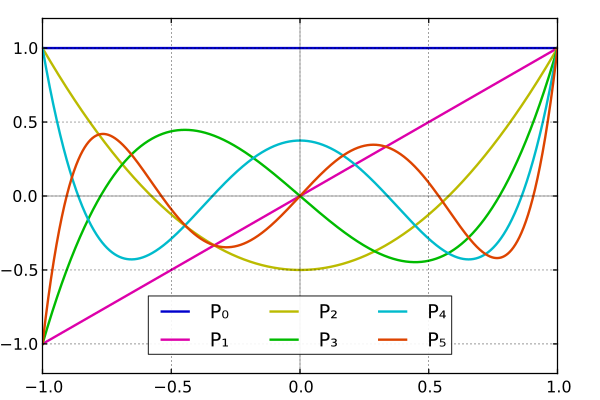
\includegraphics[width=.6\columnwidth]{lp-plot.pdf}
	\caption{Plot dei polinomi di Legendre $P_n, \ n\le 5$.}
	\label{lpplot}
\end{figure}
\subsection{Parit\`a}
Come si pu\`o notare in figura \ref{lpplot}, i polinomi di Legendre con indice pari sono pari, mentre quelli con indice dispari sono dispari.
\begin{proof}
Evidentemente, $\operatorname{deg} \big(P_n(-x)\big) = n$; usando che, per definizione $\langle P_n(x) ,Q(x) \rangle=0$ se $\operatorname{deg} (Q) < n$, allora tramite integrazione per sostituzione:
\[
\big\langle P_n(-x) , Q(x)  \big\rangle = \big\langle P_n(x) , Q(-x) \big\rangle=0
\] 
Allora deve risultare $P_n(-x) = \lambda P_n(x)$ per qualche costante $\lambda $ perch\'e sia verificato $\langle P_n(-x) , Q(x) \rangle=0$.
Usando questo, si nota che:
\[
		\lambda \langle P_n(x) , x^n \rangle= \langle P_n(-x), x^n \rangle = (-1)^n \langle P_n(-x) , (-x)^n \rangle = (-1)^n \langle P_n(x),x^n \rangle
	\]
	\[
		\Rightarrow P_n(-x) = (-1)^n P(x)
\] 
Questo dimostra che i polinomi di grado pari sono pari e quelli di grado dispari sono dispari.
\end{proof}
\subsection{La formula di Rodrigues}
Siano $P,Q : \left[ -1,1 \right] \to \mathbb{R}$ due generici polinomi in $x$; tramite integrazione per parti
\[
\int_{-1} ^{+1} P'(x) Q(x) \ dx = \big[PQ\big]_{-1} ^{+1} - \int_{-1} ^{+1} P(x) Q'(x) \ dx
\] 
si ottiene la seguente formula per il calcolo del prodotto scalare:
\begin{equation}\label{eq1}
	\langle P' , Q \rangle = \big[PQ\big]_{-1} ^{+1} - \langle P,Q' \rangle
\end{equation}
Se $(x^2 - 1 )$ divide $P$ o divide $Q$, la \ref{eq1} diventa $\langle P' , Q \rangle =  - \langle P,Q' \rangle$.
Applicando questa propriet\`a, si osserva che
\[
\left\langle \frac{d ^n}{d x^n} (x^2 - 1)^n, Q \right\rangle \propto \left\langle (x^2-1)^n , \frac{d ^n}{d x^n} Q \right\rangle
\] 
Allora:
\begin{equation}
	\operatorname{deg} (Q) < n \implies \left\langle \frac{d ^n}{d x^n} (x^2-1)^n,Q \right\rangle=0
\end{equation}
Visto che $D^n_x (X^2-1)^n$ \`e un polinomio di grado $n$, per le propriet\`a dei polinomi di Legendre, si deduce che:
\begin{equation}
	\frac{d ^n}{d x^n} (x^2-1)^n = \lambda P_n(x)
\end{equation}
Ora si vuole trovare il valore di $\lambda $; per farlo, si usa la regola di Leibniz:
\[
	\begin{split}
		\frac{d ^n}{d x^n} (x^2-1)^n &= \frac{d ^n}{d x^n} \Big[(x+1)^n (x-1)^n\Big] = \sum_{k=0}^{n} \binom{n}{k} \frac{d ^k}{d x^k}(x+1)^n \frac{d ^{n-k} }{d x^{n-k} } (x-1)^n\\
					     &=\sum_{k=0}^{n} \binom{n}{k} \frac{n!}{(n-k)!} (x+1)^{n-k} \frac{n!}{k!}(x-1)^k
	\end{split}
\] 
Da questa, si nota che per $x=1$, tutti i termini sono nulli eccetto quello per $k=0$, che sarebbe $1$; conseguentemente:
\[
	\Eval{\frac{d ^n}{d x^n} (x^2-1)^n}{x=1}{} = 2^n n!
\] 
Visto che $P_n(1) = 1$, allora si ottiene la \textit{formula di Rodrigues} per i polinomi di Legendre:
\begin{boxenv}[]
\begin{equation}
	P_n(x) = \frac{1}{n!2^n }\frac{d ^n}{d x^n} (x^2-1)^n
\end{equation}
\end{boxenv}
\subsection{L'equazione differenziale di Legendre}
Si definisce l'operatore differenziale
\begin{equation}
	L = \frac{d }{d x} \left[(1-x^2) \frac{d }{d x} \right]
\end{equation}
Assumendo che uno fra i due polinomi $P,Q : [-1,1] \to \mathbb{R}$ sia divisibile per $x^2-1$, allora si pu\`o usare $\langle P',Q \rangle= -\langle P,Q' \rangle$ per dimostrare che $L$ \`e Hermitiano:
\[
	\begin{split}
		\left\langle \frac{d }{d x} \left[ (1-x^2) \frac{d }{d x}  \right] P , Q \right\rangle &= - \left\langle (1-x^2) \frac{d }{d x} P,\frac{d }{d x} Q \right\rangle =- \left\langle \frac{d }{d x} P , (1-x^2) \frac{d }{d x} Q\right\rangle\\
		&= \left\langle P, \frac{d }{d x}\left[ (1-x^2) \frac{d }{d x}  \right] Q  \right\rangle
	\end{split}
\] 
cio\`e $\langle L[P],Q \rangle= \langle P,L[Q] \rangle$.
L'operatore $L$ mantiene il grado del polinomio, ossia $\operatorname{deg} \big(L[P]\big) = \operatorname{deg}(P) $ per il fatto che le derivate abbassano il grado di $2$ e il prodotto per $1-x^2$ lo ripristina.

Se $\operatorname{deg} (Q) < n$, allora, per $P_n$ polinomio di Legendre, si ha $\langle L[P_n], Q \rangle= \langle P_n,  L[Q] \rangle= 0$, pertanto deve valere $L[P_n] = \lambda P_n$.
Per trovare il valore di $\lambda $, si considera
\[
	\begin{split}
		\lambda \langle P_n, x^n \rangle &= \langle L[P_n], x^n \rangle= \langle P_n , L[x^n] \rangle = \left\langle P_n,(n-1)nx^{n-2} -n(n+1)x^n  \right\rangle\\
						 &=-n(n+1)\langle P_n,x^n \rangle
	\end{split}
\] 
dove si \`e eliminato il termine proporzionale a $x^{n-2} $ perch\'e ortogonale a $P_n$ per definizione.
Da questo, si conclude che $\lambda = -n(n+1)$, il che permette di ottenere due, equivalenti, equazioni differenziali per l'$n$-esimo polinomio di Legendre:
\begin{boxenv}[]
\begin{equation}
	\begin{split}
		&\frac{d }{d x} \left[ (1-x^2)\frac{d }{d x}  \right] P_n(x) + n(n+1) P_n(x) = 0\\
		\\
		&(1-x^2)P''_n(x) - 2x P'_n(x) + n(n+1) P_n(x) = 0
	\end{split}
\end{equation}
\end{boxenv}
Questa \`e nota col nome di \textit{equazione differenziale di Legendre}.
Prendendo $x=1$ in questa equazione, si ricava il valore della derivata in corrispondenza di tale valore: $P'_n(1) = n(n+1) / 2$ ({\color{red}Controllare analogia con formuladi Gauss per la somma dei primi $n$ interi}).
\subsection{Formula ricorsiva di Bonnet}
Per ricavare un'espressione che permetta il calcolo ricorsivo dei polinomi, si parte dal valutare $\langle xP_n,P_m \rangle = \langle P_n,xP_m \rangle$, che risulta nullo se $m+1 < n$.
Questo permette di concludere che $P_{n+1}=\alpha xP_n + \beta P_{n-1} + \gamma P_n $, dove $\alpha  + \beta  + \gamma = 1$ per normalizzazione.
Imponendo che i polinomi nei due membri dell'equazione abbiano stessa parit\`a, si deve prendere $\gamma=0$, per cui deve valere $\alpha  + \beta  = 1$.

Per trovare i valori di $\alpha $ e $\beta $, si ha gi\`a l'equazione $\alpha  + \beta  = 1$; inoltre, derivando e prendendo $x=1 $ nell'equazione trovata sopra:
\[
\begin{split}
	&P'_{n+1}  = \alpha (P_n + x P'_n) + \beta P'_{n-1} \\
	&\Rightarrow \frac{(n+1)(n+2)}{2} = \alpha \left[ 1 + \frac{n(n+1)}{2} \right] + \beta \frac{n(n-1)}{2}
\end{split}
\] 
da cui $\alpha = (2n+1) / (n+1)$ e $\beta = - n / (n+1)$.
Mettendo tutto insieme, si trova la \textit{formula di Bonnet}:
\begin{boxenv}[]
\begin{equation}
	(n+1) P_{n+1} (x) = (2n+1) x P_n(x) - n P_{n-1} (x)
\end{equation}
\end{boxenv}
\subsection{Funzione generatrice}

Si definisce la funzione generatrice come:
\[
g(x,t) = \sum_{n=0}^{+\infty} P_n(x) t^n
\] 
dove i polinomi di Legendre $P_n$ sono i coefficienti di una serie di potenze.
Assumendo che $\lvert t \rvert < 1$:
\[
g(1,t) = \sum_{n=0}^{+\infty} t^n = \frac{1}{1-t}\hspace{1cm} g(-1,t) = \sum_{n=0}^{+\infty} (-1)^n t^n = \frac{1}{1+t}
\] 
Ora, partendo dalla formula di Bonnet e moltiplicando per $t^n$:
\[
\begin{split}
	&(n+1) P_{n+1} (x) t^n= (2n+1) x P_n(x) t^n- n P_{n-1} (x)t^n\\
	&\Rightarrow (n+1) P_{n+1} t^n = x P_n t^n + 2nx P_n t^n - (n-1) P_{n-1} t^n - P_{n-1} t^n\\
	&\Rightarrow \frac{\partial }{\partial t} \big(P_{n+1} t^{n+1} \big) = x (P_nt^n) + 2tx\frac{\partial }{\partial t} (P_nt^n) - t^2 \frac{\partial }{\partial t} (P_{n-1} t^{n-1} ) + t(P_{n-1} t^{n-1} )\\
	&\Rightarrow \frac{\partial g}{\partial t}  = xg + 2tx \frac{\partial g}{\partial t}  - t^2 \frac{\partial g}{\partial t} + tg\\
	&\Rightarrow (1-2tx+t^2) \frac{\partial g(x,t)}{\partial t} = (x-t) g(x,t)
\end{split}
\] 
dove per la terza implicazione, si \`e sommato su $n$. 
Ora, chiamando $(1-2tx+t^2) = h(x,t)$, che \`e tale per cui $\partial _t h = 2(t-x)$, si ottiene:
\[
	h(x,t) \frac{\partial g(x,t)}{\partial t} = -\frac{1}{2}g(x,t)\frac{\partial }{\partial t} h(x,t) \implies \frac{1}{g(x,t)}\frac{\partial g(x,t)}{\partial t} = -\frac{1}{2h(x,t)} \frac{\partial h(x,t)}{\partial t} 
\] 
Integrando ambo i membri, si ottiene
\[
	\ln \big(g(x,t)\big) = - \frac{1}{2} \ln\big(h(x,t)\big) + c(x) \implies g(x,t) = \frac{e^{c(x)} }{\sqrt{h(x,t)} }
\] 
Per trovare $c(x)$, si usa che $g(x,0) = 1 \Rightarrow c(x) = 0$. 
Complessivamente, la funzione generatrice \`e:
\begin{boxenv}[]
\begin{equation}
	g(x,t) = \frac{1}{\sqrt{1-2tx+t^2} }
\end{equation}
\end{boxenv}































\newpage
\section{Da fare}


\begin{itemize}
	\item Partire dal problema di Laplace in coordinate polari. 
	\item Definire l'operatore differenziale $L[P]$ nell'equazione differenziale dei polinomi.
	\item Vedere cosa significa autoaggiunto nel senso di Sturm-Liouville.
	\item Definire in generale il prodotto scalare per spazi di funzioni.
	\item Trarre da questo che il prodotto scalare deve avere peso costante e unitario.
	\item Motivare la scelta dell'intervallo $[-1,1]$.
\end{itemize}
\end{document}

